% !TeX program = xelatex
\documentclass[
  convert={density=500, size=600, outext=.png}, 
  border=2pt
]{standalone}

\usepackage{fontspec}
\defaultfontfeatures{Ligatures={NoCommon,%
			NoDiscretionary,%
			NoHistoric,%
			NoRequired,%
			NoContextual}}
\setsansfont{Carlito}[%
	SmallCapsFeatures={Letters=SmallCaps},%
	SmallCapsFont={Roboto},%
	ItalicFeatures={SmallCapsFont=Roboto-Italic},%
	BoldFeatures={SmallCapsFont=Roboto-Bold},%
	BoldItalicFeatures={SmallCapsFont=Roboto-BoldItalic}%
]

\usepackage{tikz}
\usepackage{tikz-cd}
\usetikzlibrary{%
	calc,%
	arrows.meta,%
	arrows,%
	automata,%
	overlay-beamer-styles,%
	snakes,%
	shapes.arrows,%
	shapes.geometric,%
	shapes.symbols,%
	fit,%
	positioning,%
	decorations.pathreplacing,%
	backgrounds,%
}
\tikzset{
	>=Triangle,%
	nodes={align=center},%
	comp/.style={%
			draw,%
			rectangle,%
			very thick,%
			rounded corners,%
			minimum width=2.5cm,%
			minimum height=1cm,%
			fill=white},%
	input/.style={draw,%
			rectangle,%
			thick,%
			minimum width=2.5cm,%
			minimum height=1cm,%
			fill=white},%
	classnode/.style={%
			fill=cgreenlight,%
			rectangle,%
			draw,%
			inner xsep=0},%
	interfacenode/.style={%
			fill=corangelight,%
			rectangle,%
			draw,%
			inner xsep=0},%
	abstractclassnode/.style={%
			fill=cbluelight,%
			rectangle,%
			draw,%
			inner xsep=0},%
	inlinenode/.style={%
			inner xsep=.5cm,%
			minimum height=.6cm},%
}

\definecolor{reddy}{RGB}{172, 0, 51}
\definecolor{dkred}{rgb}{.6, 0, 0}
\definecolor{dkgreen}{rgb}{0, .5, 0}
\definecolor{dkblue}{rgb}{0, 0, .5}
\definecolor{cred}{RGB}{219, 68, 55}
\definecolor{credlight}{RGB}{250, 227, 225}
\definecolor{cgreen}{RGB}{3, 148, 77}
\definecolor{cgreenlight}{RGB}{209, 251, 230}
\definecolor{cblue}{RGB}{2, 119, 189}
\definecolor{cbluelight}{RGB}{208, 237, 254}
\definecolor{corange}{RGB}{173, 128, 2}
\definecolor{corangelight}{RGB}{253, 219, 123}
\newcommand{\cblue}[1]{\textcolor{cblue}{#1}}
\newcommand{\bfcblue}[1]{\textcolor{cblue}{\textbf{#1}}}
\newcommand{\cred}[1]{\textcolor{cred}{#1}}
\newcommand{\bfcred}[1]{\textcolor{cred}{\textbf{#1}}}
\newcommand{\cgreen}[1]{\textcolor{cgreen}{#1}}
\newcommand{\bfcgreen}[1]{\textcolor{cgreen}{\textbf{#1}}}
\newcommand{\corange}[1]{\textcolor{corange}{#1}}
\newcommand{\bfcorange}[1]{\textcolor{corange}{\textbf{#1}}}
\newcommand{\interfacename}[1]{\underline{\textbf{\textit{#1}}}}
\newcommand{\absclassname}[1]{\textbf{\textit{#1}}}
\newcommand{\classname}[1]{\textbf{#1}}

\usepackage{amsmath}
\usepackage{amsfonts}
\usepackage{amssymb}

\usepackage{silence}
\WarningsOff*


\begin{document}
\sffamily

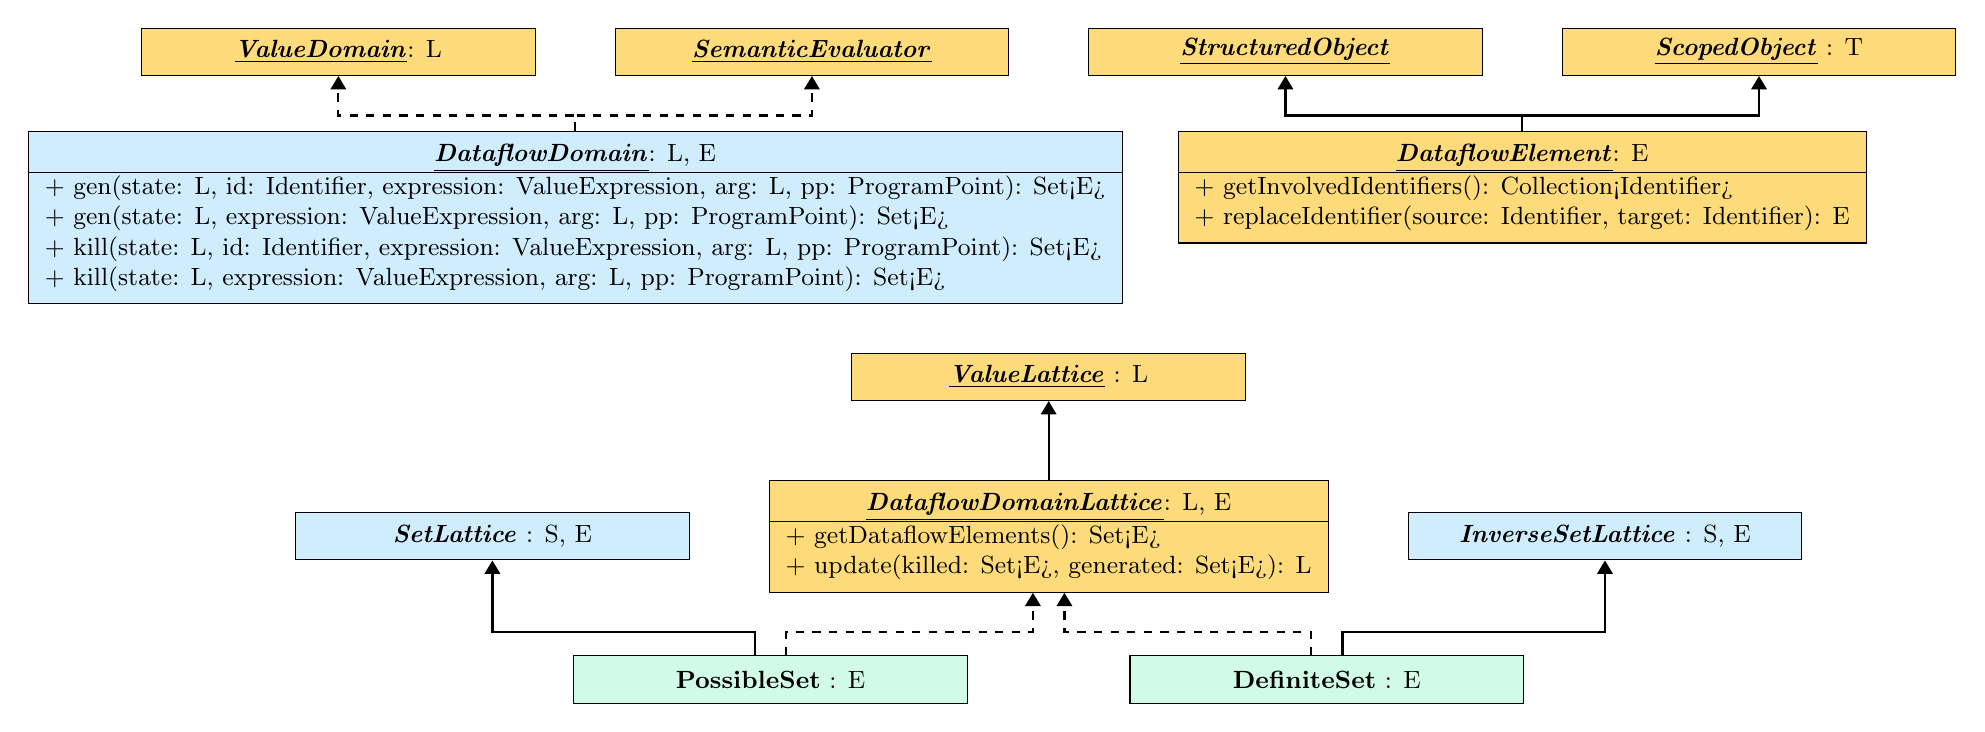
\begin{tikzpicture}[nodes={font={\small}, minimum width=5cm, minimum height=.6cm}]%
	\node[interfacenode, inlinenode] (vd) {\interfacename{ValueDomain}: L};
	\node[interfacenode, inlinenode] (se) [right=of vd] {\interfacename{SemanticEvaluator}};
	\node[abstractclassnode] (dd) [below=of $(vd)!0.5!(se)$] {\begin{tabular}{l}
			\multicolumn{1}{c}{\interfacename{DataflowDomain}: L, E}                                        \\
			\hline
			+ gen(state: L, id: Identifier, expression: ValueExpression, arg: L, pp: ProgramPoint): Set<E>  \\
			+ gen(state: L, expression: ValueExpression, arg: L, pp: ProgramPoint): Set<E>                  \\
			+ kill(state: L, id: Identifier, expression: ValueExpression, arg: L, pp: ProgramPoint): Set<E> \\
			+ kill(state: L, expression: ValueExpression, arg: L, pp: ProgramPoint): Set<E>                 \\
		\end{tabular}};

	\node[interfacenode, inlinenode] (so) [right=of se] {\interfacename{StructuredObject}};
	\node[interfacenode, inlinenode] (sO) [right=of so] {\interfacename{ScopedObject} : T};
	\node[interfacenode] (de) [below=of $(so)!0.5!(sO)$] {\begin{tabular}{l}
			\multicolumn{1}{c}{\interfacename{DataflowElement}: E}         \\
			\hline
			+ getInvolvedIdentifiers(): Collection<Identifier>             \\
			+ replaceIdentifier(source: Identifier, target: Identifier): E \\
		\end{tabular}};

	\node[interfacenode, inlinenode] (vl) [below=of $(dd.south)!0.5!(de.south)$] {\interfacename{ValueLattice} : L};
	\node[interfacenode] (ddl) [below=of vl] {\begin{tabular}{l}
			\multicolumn{1}{c}{\interfacename{DataflowDomainLattice}: L, E} \\
			\hline
			+ getDataflowElements(): Set<E>                                 \\
			+ update(killed: Set<E>, generated: Set<E>): L                  \\
		\end{tabular}};
	\node[abstractclassnode, inlinenode] (sl) [left=of ddl] {\absclassname{SetLattice} : S, E};
	\node[abstractclassnode, inlinenode] (isl) [right=of ddl] {\absclassname{InverseSetLattice} : S, E};
	\node[classnode, inlinenode] (ps) [below=of $(sl.south)!0.5!(ddl.south)$] {\classname{PossibleSet} : E};
	\node[classnode, inlinenode] (ds) [below=of $(isl.south)!0.5!(ddl.south)$] {\classname{DefiniteSet} : E};

	\draw[->, thick, dashed] (dd) |- ($(vd.south)+(0,-0.5)$) to (vd);
	\draw[->, thick, dashed] (dd) |- ($(se.south)+(0,-0.5)$) to (se);
	\draw[->, thick] (de) |- ($(so.south)+(0,-0.5)$) to (so);
	\draw[->, thick] (de) |- ($(sO.south)+(0,-0.5)$) to (sO);
	\draw[->, thick] (ddl) to (vl);
	\draw[->, thick, dashed] ($(ps.north)+(0.2,0)$) to ($(ps.north)+(0.2,0.3)$) -| ($(ddl.south)+(-0.2,0)$);
	\draw[->, thick] ($(ps.north)+(-0.2,0)$) to ($(ps.north)+(-0.2,0.3)$) -| (sl);
	\draw[->, thick, dashed] ($(ds.north)+(-0.2,0)$) to ($(ds.north)+(-0.2,0.3)$) -| ($(ddl.south)+(0.2,0)$);
	\draw[->, thick] ($(ds.north)+(0.2,0)$) to ($(ds.north)+(0.2,0.3)$) -| (isl);
\end{tikzpicture}

\end{document}
